\chapter{Experimental design and procedure}
\label{chap:experimentation}

\section{Participants}
\label{sec:expparticipants}

The total number of participants was three small children, all female, two belonging to the target age range (15 and 24 months of age) and one younger (9 months of age). Their parents did not report any diagnosis of clinical conditions or vision problems related to the children.
In addition, the author made a pilot test on himself in order to provide the “ideal” eye tracking record set, which is used a reference for the comparison on the experimental group record sets. The participant profiles is shown in Tab.~\ref{tab:participants}.

\begin{table}[h]
   \centering
   \begin{tabular}{@{}c@{\hspace{.5cm}}c@{}}
       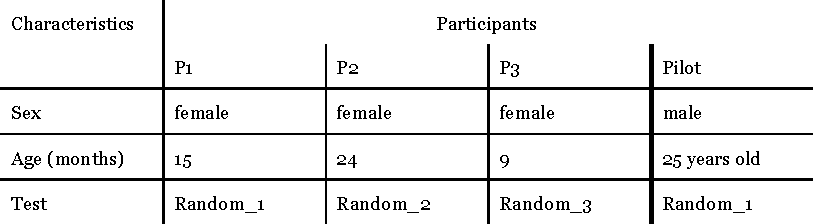
\includegraphics[page=1,width=1\textwidth]{figures/tables/table_3.pdf}
   \end{tabular}
 \caption{Participants profiles.}
 \label{tab:participants}
\end{table}

The recruitment was done by convenience sampling, with a snowball sampling approach \citep[pp. 496, 506]{baxter2015understanding}, looking for parents within the network of acquaintances of the researchers who might have had children in the target age range. This technique was chosen due the following reasons:
\begin{itemize}
    \item The necessity of collecting a trustworthy informed consent, and therefore clarifying in detail the aims of the experimentation. Due to the fact that the research involves concepts related to ASD, it was of utmost importance to clarify that no evaluation would have been carried out on the children’s performance. This task demanded for personal communication.
    \item The importance of establishing a relationship of trust with the parents in order to conduct experiments on their babies. The very young age of the participants makes them a sensitive experimental group. Moreover, eye tracking technologies and research methods are not to be expected to be known by parents as general knowledge. Also this task demanded for personal communication.
    \item The objectives of the experiments did not include statistical significance. Therefore a more personal approach allowed to establish the necessary collaboration with the parents, and involve them as partners (and also stakeholders) in the research. Their help was indeed fundamental.
\end{itemize}

Originally, only two participants were identified (P1 and P2), who belonged to the target age group. P3 became a participant since she was present at the experimental facility, and her parent proposed and allowed for doing the experiment. This provided the opportunity to test the procedure on children even younger than the target age range of 12-24 months.




\section{Apparatus}
\label{sec:expapparatus}

The eye tracker used in the experiments is the SMI\textsuperscript{\textregistered} RED250mobile\texttrademark, produced by SensoMotoric Instruments GmbH (Teltow, Germany). It is a remote model, which is to be placed underneath a display monitor and it casts infrared light towards the pupil of the subject in order to track the movement of the eyes. Since it does not produce sounds or movements, and it does not require the subject to wear additional equipment, it gets inconspicuous and unobtrusive. The sample rate was set to 250 Hz, which it is sufficient for tracking saccades, smooth pursuit movements and fixations. It can also track blinks and pupil dilation. The eye tracker software and its experiment suite (SMI Experiment Suite\texttrademark 3.6) are installed on a laptop computer (7th Generation Intel\textsuperscript{\textregistered} Core\texttrademark i7 processor 2.50 GHz; 8GB RAM, NVIDIA® Quadro\texttrademark graphic card with 2GB dedicated memory; 32 bit colors; 15.6-inch diagonal anti-glare LED-backlit display, resolution 1920x1080px, 60Hz; the monitor size covers ~39 degrees of visual angle horizontally and ~22 degrees vertically, when it is viewed at 50 cm of distance). This setup is powerful and portable enough to be carried around and used in different settings, according to where the evaluation takes place, either in an home environment, in a clinical structure, or wherever the child feels more at ease.
The computer was controlled at distance by using a portable keyboard connected to the experiment computer by a long USB cable. This allowed the researchers to stay out of the participant’s sight and at the same time controlling the progress of the experiment. A scheme of the setting is shown in Fig.~\ref{fig:settingscheme}.

\begin{figure}[h]
  \centering
  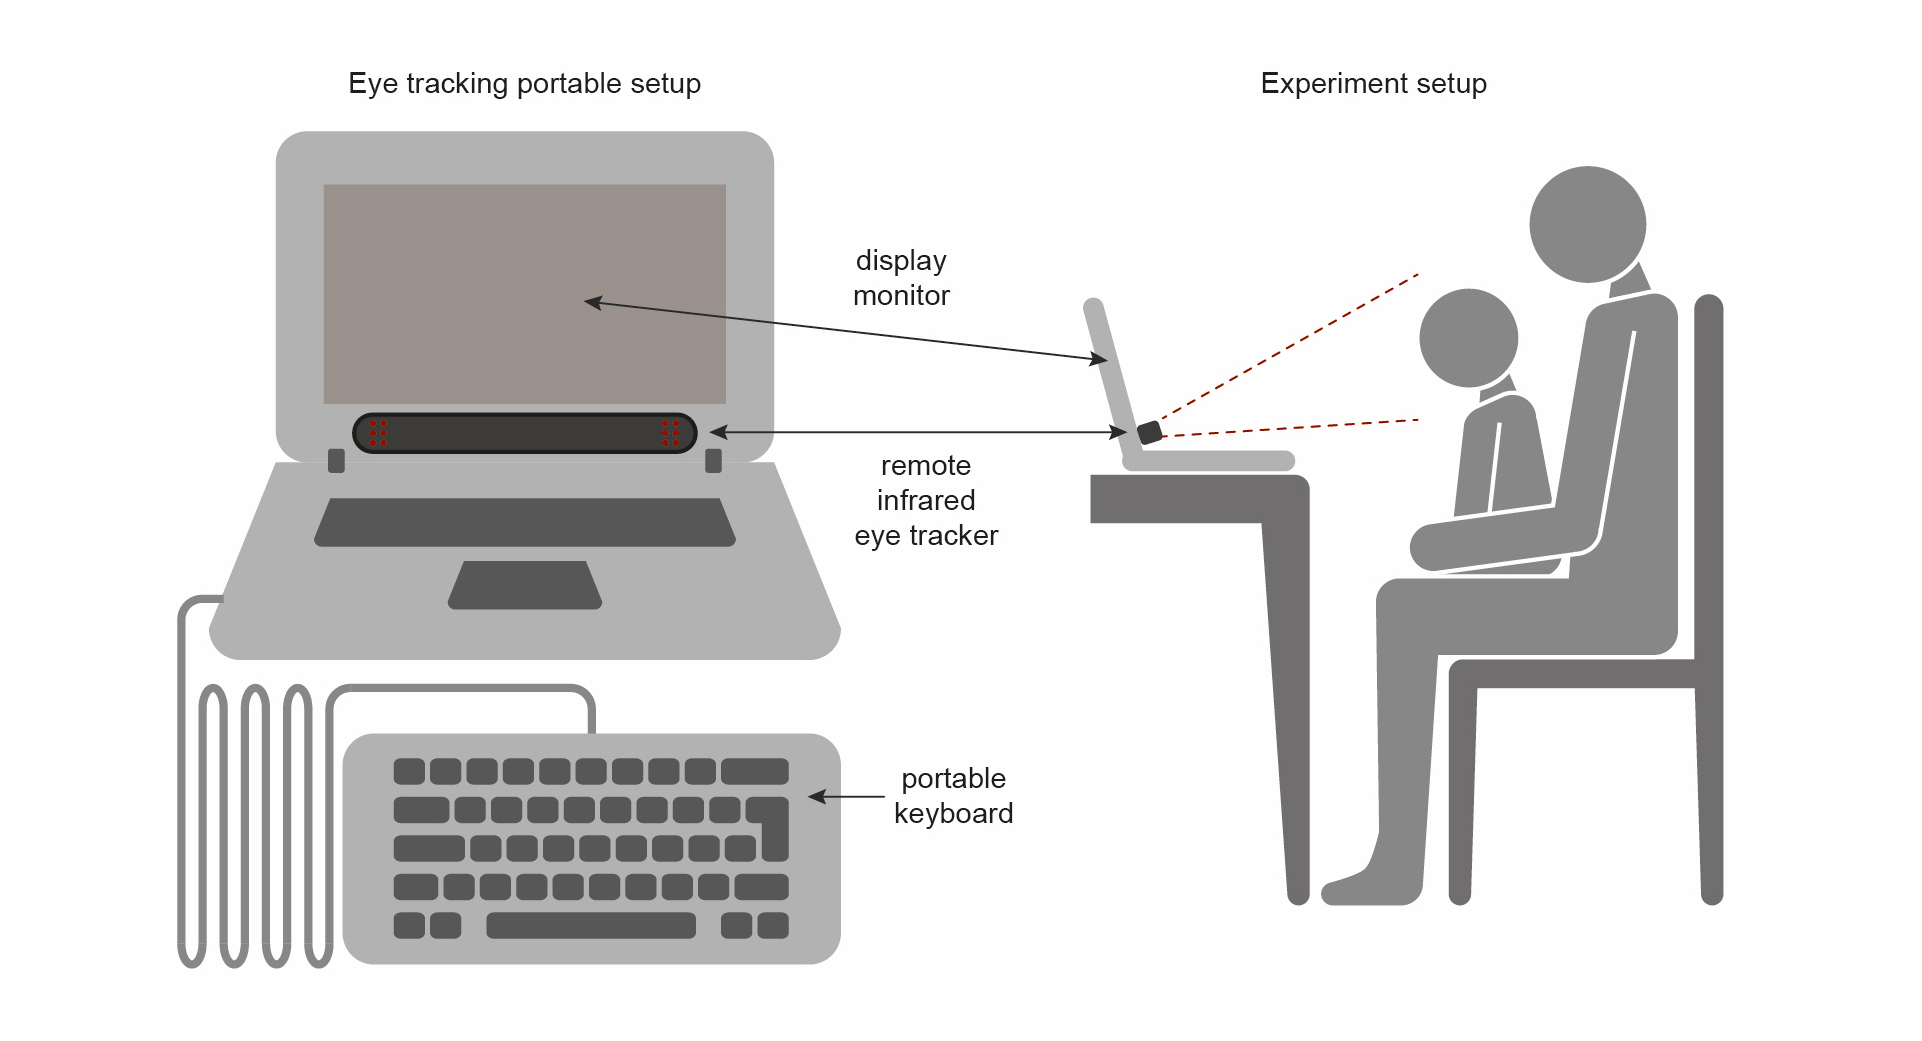
\includegraphics[width=1\textwidth]{figures/setting-01.jpg}
  \caption[Experiment setting scheme]{Scheme of the experiment equipment and setting.}
  \label{fig:settingscheme}
\end{figure}

No video recordings were set up in order to capture the events happening during the experiment, due to a couple of reasons. The agreement between the researchers and the parents of the participant children was to keep all the information related to the experiment completely anonymized. This key point in the informed consent agreement was particularly important due to the potential for the research to uncover in the future possible clinical conditions of the children. Therefore, protecting the children’s identity was of primary importance, regardless the confidentiality obligation for the researchers. Adding a video recording tool could have prevented the parents to decide to participate in the study. Moreover, a tripod and a camera could have revealed to be an invasive equipment for the home setting. Adding even more technical equipment in addition to the eye tracker and its computer could have made the setting too cluttered, and also would have required an assistant to operate it, making the environment even more crowded. For these reasons the researcher considered having video recorders not to be ideal, even if they would provide a noticeable amount of richer qualitative data, which could have been useful for deepening the analysis on the applicability of the procedure on small children.




\import{chapters/}{stimuli.tex}




\section{Experiment setting and procedure}
\label{sec:expsetting}

The research protocol for the study follows the guidelines provided by \cite{sasson2012children} for conducting eye tracking studies on young children with ASD, and by \cite[pp. 98-101]{rubinchisnell2008hout} for arranging experiment sessions at a user’s site and the preparation of a minimalist portable test lab.

The informed consent form for the participation in the study and the research protocol document follow more or less the templates provided by the \cite{rek2017templates}(REK), which are suitable for medical-related research. The detailed documents are both available in Appendix ~\ref{app:consentformNorsk} and \ref{app:researchprotocol}. The research protocol was shared and read by the researcher and the assistant before conducting the experiments.

The project proposal and the research protocol has been submitted to REK and, given the purpose of the project to just investigate the feasibility of the procedure and to not generate statistical results, REK notified that the project is not covered by the scope of the Health Research Act. Therefore, their approval was not necessary.

The experiments took place at a private home. Two attempts were made in order to find a spot in the home which was suitable enough to have good calibration, for a couple of reasons:
\begin{enumerate}
    \item The ambient illumination, mainly coming from the sunshine filtering from the windows during a very sunny and hot day, was too bright in the first location. The calibration was failing repeatedly most likely due to the fact that the pupil size of the children was too small due to physiological constriction.
    \item The geometry of the face of small babies is significantly different than the one from adults (i.e. the the pupillary distance is lower), therefore it is possible that the eye tracker software has troubles in detecting the children’s pupils correctly.
\end{enumerate}

\begin{figure}[h]
  \centering
  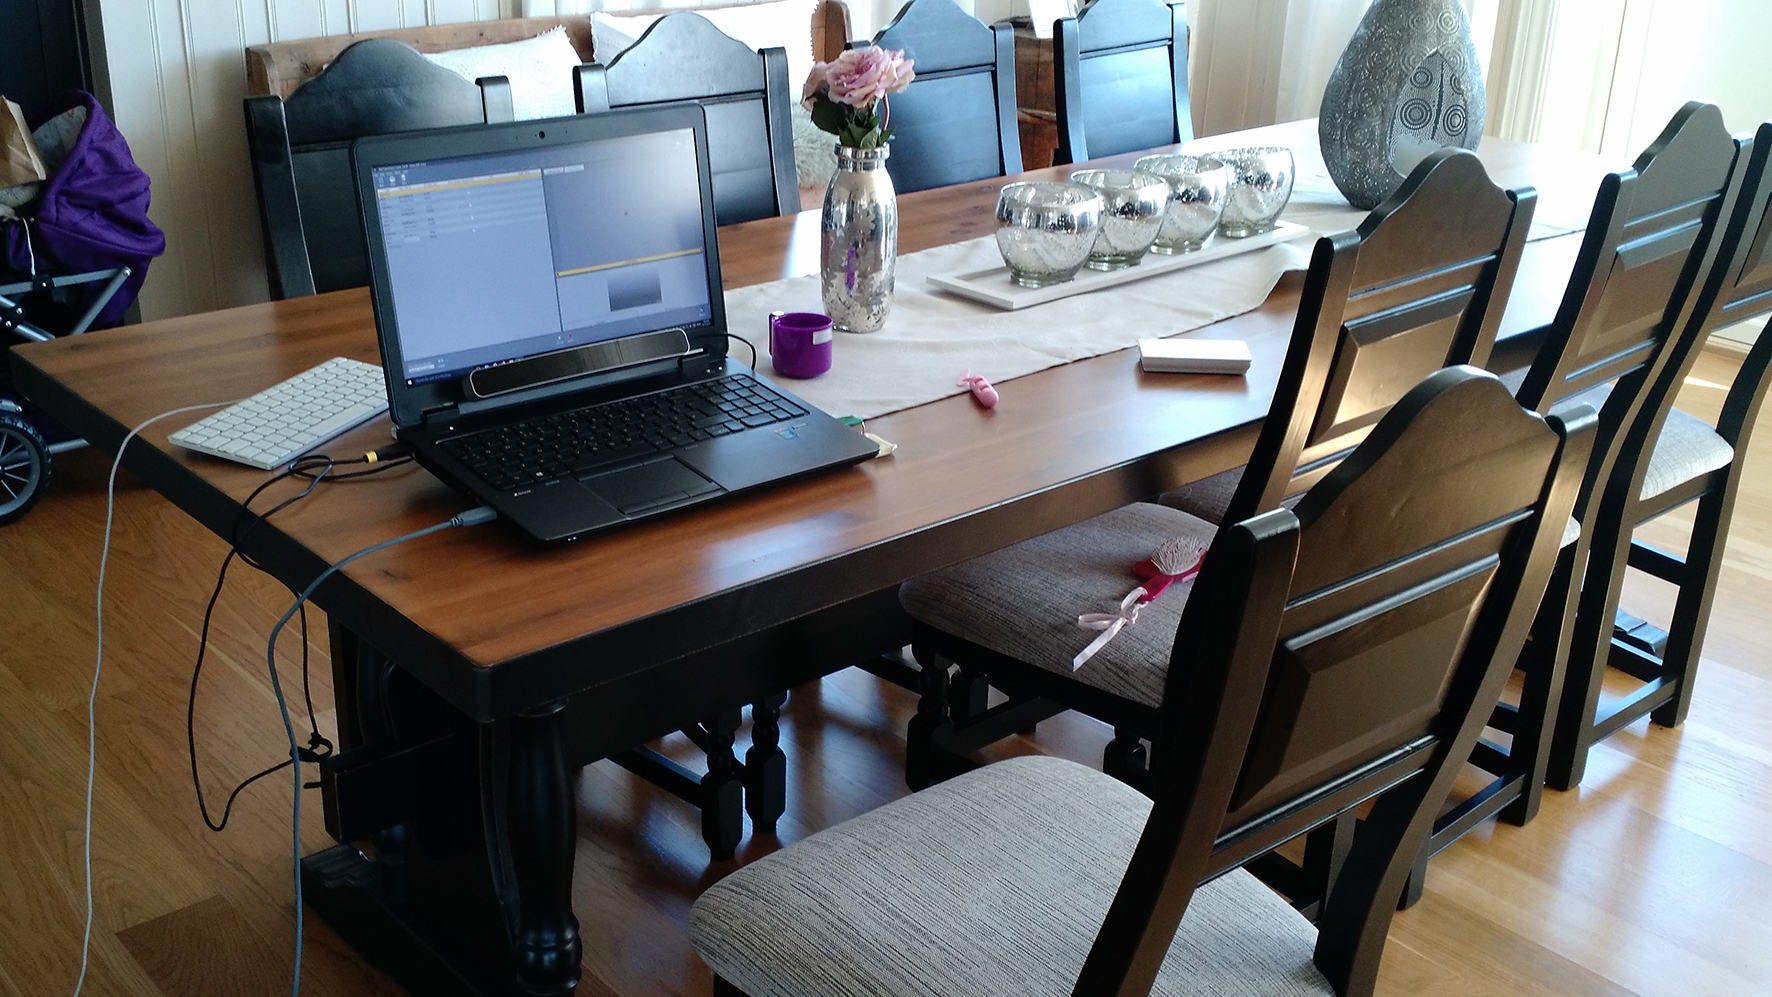
\includegraphics[width=.8\textwidth]{figures/settingphoto.jpg}
  \caption[Experiment setup]{Experiment setup in the home environment}
  \label{fig:setupphoto}
\end{figure}

The second location (Fig.~\ref{fig:setupphoto}), with dimmer ambient lightning, proven to be ideal for calibration. The location was still not fully isolated from distractions, and sometimes it was playfully noisy, with children running around. However, this kind of environment probably contributed to make feel the whole situation more relaxed and near to the everyday life of the children, which can be regarded as a positive feature.
As predictable, all the children were easily distracted by the presence of the researchers, as probably they were new people in a known environment and therefore more interesting than the experiment equipments. Even if the researchers stayed out of sight, controlling the computer remotely, every small movement or noise they made captured the children’s attention.

Before the experiments all the children were playing outside in the sun with their mothers and then during the experiments they were sitting indoors watching videos on a computer. Probably the change in the settings was pretty abrupt, and it might have impacted on the children’s willingness to follow carefully the experiment from the beginning to the end.

The detailed research protocol available in Appendix~\ref{app:researchprotocol} shows the timing and the duration of the phases of the experiment and the succession of the stimuli an interstimulus material. Here it follows a summary.

The experiment consisted of different phases:
\begin{enumerate}
    \item Introduction and setup: The caregiver is provided with a recap of the experimental procedure and an informed consent form. Then she take a seat on a chair in front of the screen at an adequate distance, keeping the child on her lap.
    \item Calibration: The researchers check if the eye tracker is detecting the child’s pupils. The caregiver is asked to wear sunglasses, in order to prevent the eye tracker to detect her eyes. When the caregiver feels that she and her child are comfortable and ready to start, a first semi-automated calibration routine is shown on the display monitor. The researchers position themselves out of the child’s field of sight, using the portable keyboard to control the experiment software.
    \item Visualization: The series of stimuli and interstimulus materials is shown, following the sequence shown in Appendix~\ref{app:researchprotocol}. The eye tracker records the data only during the stimulus presentation. The procedure is semi-automated, during which the researcher can move forward if needed by using the portable keyboard.
    \item Conclusion: When the series of stimuli is over, a message is displayed on the display monitor and the test is ended. The eye tracker recordings are saved in the experiment software.
\end{enumerate}

During the experiment, it was not possible to control constantly if the children’s eyes were at 50 cm of distance from the eye tracker (which is the distance assumed in the visual stimuli codes). It was ranging up to 60-65 cm, rendering the sizes of the targets visually smaller than planned.
